\section{Auswahl des Frameworks}%\label{sec:08_02_Auswahl-des-Frameworks}
Bei der Implementation des Frontends bestand der erste Schritt in der Auswahl des Frameworks. Die drei betrachteten Kandidaten waren Vue.js, Angular und React.

\begin{figure}[hbt!]%
  \centering
  \subfigure{
  
\includegraphics[width=3cm]{images/08-Benutzeroberfläche/08-Angular_logo.png}
  }%
  \qquad
  \subfigure{
  
\includegraphics[width=3cm]{images/08-Benutzeroberfläche/08-Vue_logo.png}
  }%
  \qquad
  \subfigure{
\includegraphics[width=4cm]{images/08-Benutzeroberfläche/08-react_logo.png}}%
  \caption{Logos der zur Auswahl stehenden Frameworks}%
\end{figure}

Nach erster Recherche wurde klar, dass alle Frameworks in der Lage sind moderne und stabile Webseiten zu erstellen. Sie unterstützen alle diverse Bibliotheken zur Visualisierung und bieten die Funktionalitäten die geplanten Inhalte umzusetzen. Da die drei Frameworks die technischen Anforderungen gleichmäßig erfüllen, konnten wir persönliche Kriterien aufstellen um eine Entscheidung zu treffen. 
Das erste Kriterium bestand in der aktuellen Nachfrage in der Wirtschaft. Dazu haben wir die Menge der Suchanfragen nach dem jeweiligen Skill in unterschiedlichen Bereichen untersucht. Angefangen haben wir mit den Jobbörsen und Business Social Networks.

\begin{figure}[hbt!]%
  \centering
  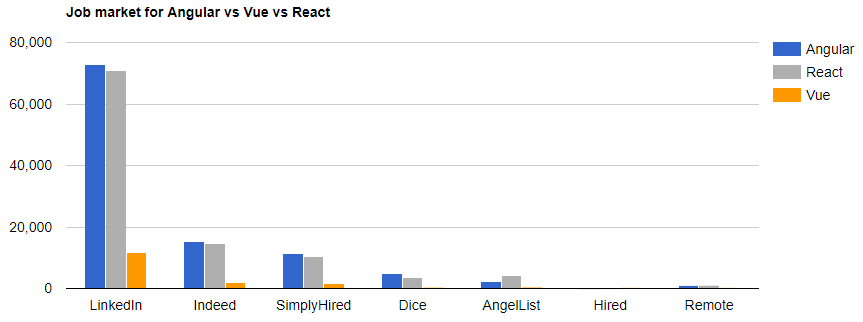
\includegraphics[width=14cm]{images/08-Benutzeroberfläche/08-jobbörsen-anfragen.PNG}
  \caption{Vergleich der Suchanfragen in Jobbörsen und Business Social Networks}%
\end{figure}

Hier ist klar, dass die Industrie mehr an den Frameworks React und Angular interessiert ist. Um die allgemeine Meinung besser einschätzen zu können haben wir die Google Trending Suchanfragen der verglichen. 

\begin{figure}[hbt!]%
  \centering
  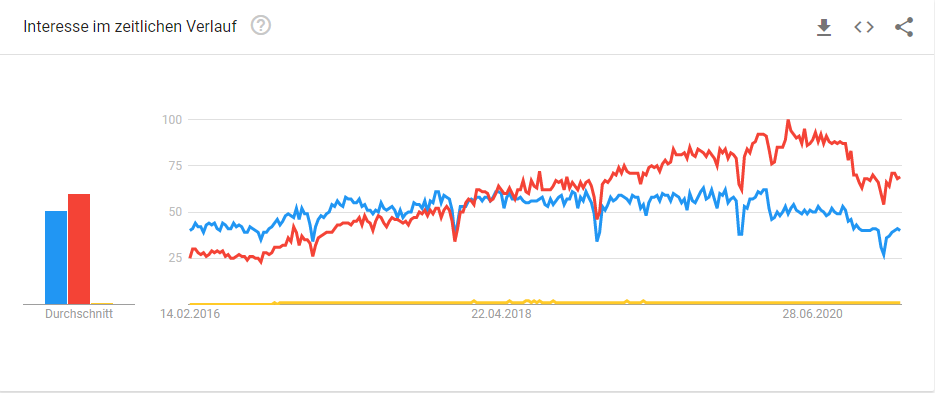
\includegraphics[width=14cm]{images/08-Benutzeroberfläche/08-google_trending.PNG}
  \caption{Vergleich der Google Trending Suchwörter}%
\end{figure}

Auch hier stehen Angular und React weit vor den Anfragen von, sodass wir uns zwischen diesen beiden entscheiden mussten. Als letztes Kriterium haben wir die aktuellen Github Statistiken der Frameworks verglichen um einen Eindruck für die Community und dessen Aktivität zu erhalten.

\begin{figure}[hbt!]%
\centering
  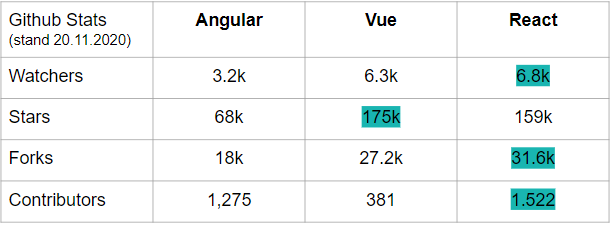
\includegraphics[width=14cm]{images/08-Benutzeroberfläche/08-github_stats.PNG}
  \caption{Vergleich der Github Statistiken der Frameworks}%
\end{figure}

Unter Berücksichtigung aller Kriterien haben wir uns für die Entwicklung der Website mit React entschieden.